\clearpage
\section{Preliminary research}

\subsection{GPS theory}

\textit{"The Global Positioning System (GPS) is a space-based satellite navigation system that provides location and time information in all weather conditions, anywhere on or near the Earth where there is an unobstructed line of sight to four or more GPS satellites. The system provides critical capabilities to military, civil, and commercial users around the world. The United States government created the system, maintains it, and makes it freely accessible to anyone with a GPS receiver."\cite{GPS1}}

The GPS satellites each carry an atomic clock and positions the user when connected to 4 or more satellites. The satellites measure the time it takes for the signal to go back and forth between the satellites and a GPS receiver\cite{GPS1}. There is also a space "GPS" system in development, that would use the X-ray signal from dying stars to give you the exact location in space with an error rate of about 5km\cite{GPS2}.

Either of those systems would not be beneficial for our project in space, since we would need a high-accuracy location of each picture we take to make a map and a model for navigation purposes. Later in the future when people will \textit{hypothetically} be moving to Mars, another GPS-like system would have to be put in place up for navigation purposes. For now, we would need to use encoders and short-to-medium range, high-accuracy signals. But these signal systems needs to be different for every planet we would go to.  

\subsection{Photogrammetry theory}

\textit{"Photogrammetry is the practice of determining the geometric properties of objects from photographic images. This is done by comparing and matching pixels or reference points across a series of photos."\cite{Photogrammetry}}

As a simple example, a map can be constructed from a series of images by overlaying them in such a way that the areas the pictures have in common, overlap. The distance between two points that lie on a plane parallel to the photographic image plane can be determined by measuring their distance on the image, if the scale (s) of the image is known. This is done by multiplying the measured distance by $1/s$\cite{photo}.

Algorithms for photogrammetry typically attempt to minimize the sum of the squares of errors over the coordinates and relative displacements of the reference points. This minimization is known as bundle adjustment and is often performed using the \textit{Levenberg–Marquardt algorithm}\cite{photo}.

Photogrammetry could also be used in our project with an AUV or a rover. There is no need for outdoor reference points to make the 3D model. But this technology is much more complicated to set-up and maintain without an outside assistance, which is a major inconvenience when used for space exploration. It would also take a large quantity of pictures in a high resolution, so in turn more space on hard drives are needed. The algorithm needs to create the 3D model from the pictures, which will need a lot of computing power and memory. So doing on board rendering would be really hard and resource consuming for smaller computing units.

For higher resolution maps and more detailed the use of photogrammetry is beneficial, But to start with, it would be easier to take another approach. %TODO: Maybe elaborate on this other approach?! 
%Thomas: I think it should just be deleted.
%gustavo: agree. having it wouldn't add anything really
\subsection{Reference points theory}

To make a 2D or 3D map, a reference point is needed. It can be GPS positions of every picture taken or it can also be by comparing two pictures and overlapping them. It is also possible to combine both options, but with the lack of GPS in space and the cost of memory and power to make an overlapping 3D map, another solution is needed. For an example, Mars has a thin atmosphere, so using sound sensors could be a possibility. The sensors would need to be calibrated to work correctly on Mars, since there is a difference in the speed of sound. Other sensors such as light (X-ray, laser, etc.) can also be used. That would mean setting up and array of sensors, so a rover or an AUV could potentially connect to them and know their position. The use of encoders and the wheels of the rover is also another solution, but this requires error calculation in it, since sometimes the tires will attempt to move in a circle but there is no traction to help create the movement\cite{reference}.

\subsection{SLAM}

Simultaneous Localization and Mapping (SLAM) is a particular method used to construct maps. In SLAM, the mapping device maps its environment whilst simultaneously keeping track of its location within that map, hence the name. SLAM is used mostly in autonomous vehicles that need to traverse some terrain without any prior information about it. More precisely, SLAM is a combination of algorithms, most notably \textit{Kalman filtering}, that all relate to either mapping or navigation. The specifics of these algorithms are too complex for the purpose and timescale of this project.

\subsection{Sensors}
\subsubsection{Pressure Based}
Pressure-based sensors work by simply measuring how much pressure there is in a point in space. They can be used to measure the vertical distance between two points in a planet with an atmosphere\cite{barometric1}\cite{barometric2}. By combining height information with the data gathered by other sensors, it is possible to create a crude three-dimensional map.

\subsubsection{Image Based}
Image-based sensors are often cameras or camera-like equipment. The pictures that the sensor takes, must be mathematically processed to yield any useful data. The two most common types of image sensors are stereoscopic and projected image sensors.

A projected image sensor is where some known image is projected on the environment (a grid, for example), then a camera takes a picture. Since the projection is known, it is simple to detect the distance of an object on the image, based on what the projection looks like. This method is limited to how fine the projected image is.

Stereoscopy, also known as stereo-photogrammetry, is more complicated, but also more reliable. Two photos of the same scene, but from different vantage points, are taken. Small sections of one of the images are taken, and overlayed onto the other image. By finding the place on the other image where the small section fits, the algorithm can determine the depth of each pixel in that subsection. This procedure is repeated until the whole image has been processed.

\subsection{Optical-flow sensor}
An Optical-flow sensor is a camera mounted on a PCB board that compares changes in pixels to look out for drift and movement in a system. The concept is the same as your computer mouse follows. It will tell you the movement of your vehicle in a $XY$-grid.

\subsection{Rangefinder}
A rangefinder is a device that measures the distance between itself, and a point at a certain distance away from it. Rangefinders work based on the principle that the speed of an object is defined to be \textit{distance travelled over time travelled}, which means that the \textit{distance travelled} is the speed of an object times the amount of time it travelled. To put this in math terms: \(v=d/t\) or \(d=t*v\).

Most rangefinders work on either sound or light. Both sound- and light-based rangefinders work by emitting a pulse in a specific direction, and counting how long it takes for the pulse to come back. Since the pulse has travelled back and forth, the distance is calculated as \(\frac{1}{2}*v*t\), where \(v\) is the speed of the pulse, and \(t\) is the time between the emission and the detection.

The pulse will travel from the rangefinder, straight towards whatever object is in front of it. Often, the pulse is not normal to the object it hits; meaning that the pulse is at an angle relative to the object, so the pulse will not reflect back to the rangefinder. However, a small portion of the pulse will scatter upon impact, meaning the rangefinder might still detect the pulse once it comes back.

\begin{figure}[H]
	\centering
	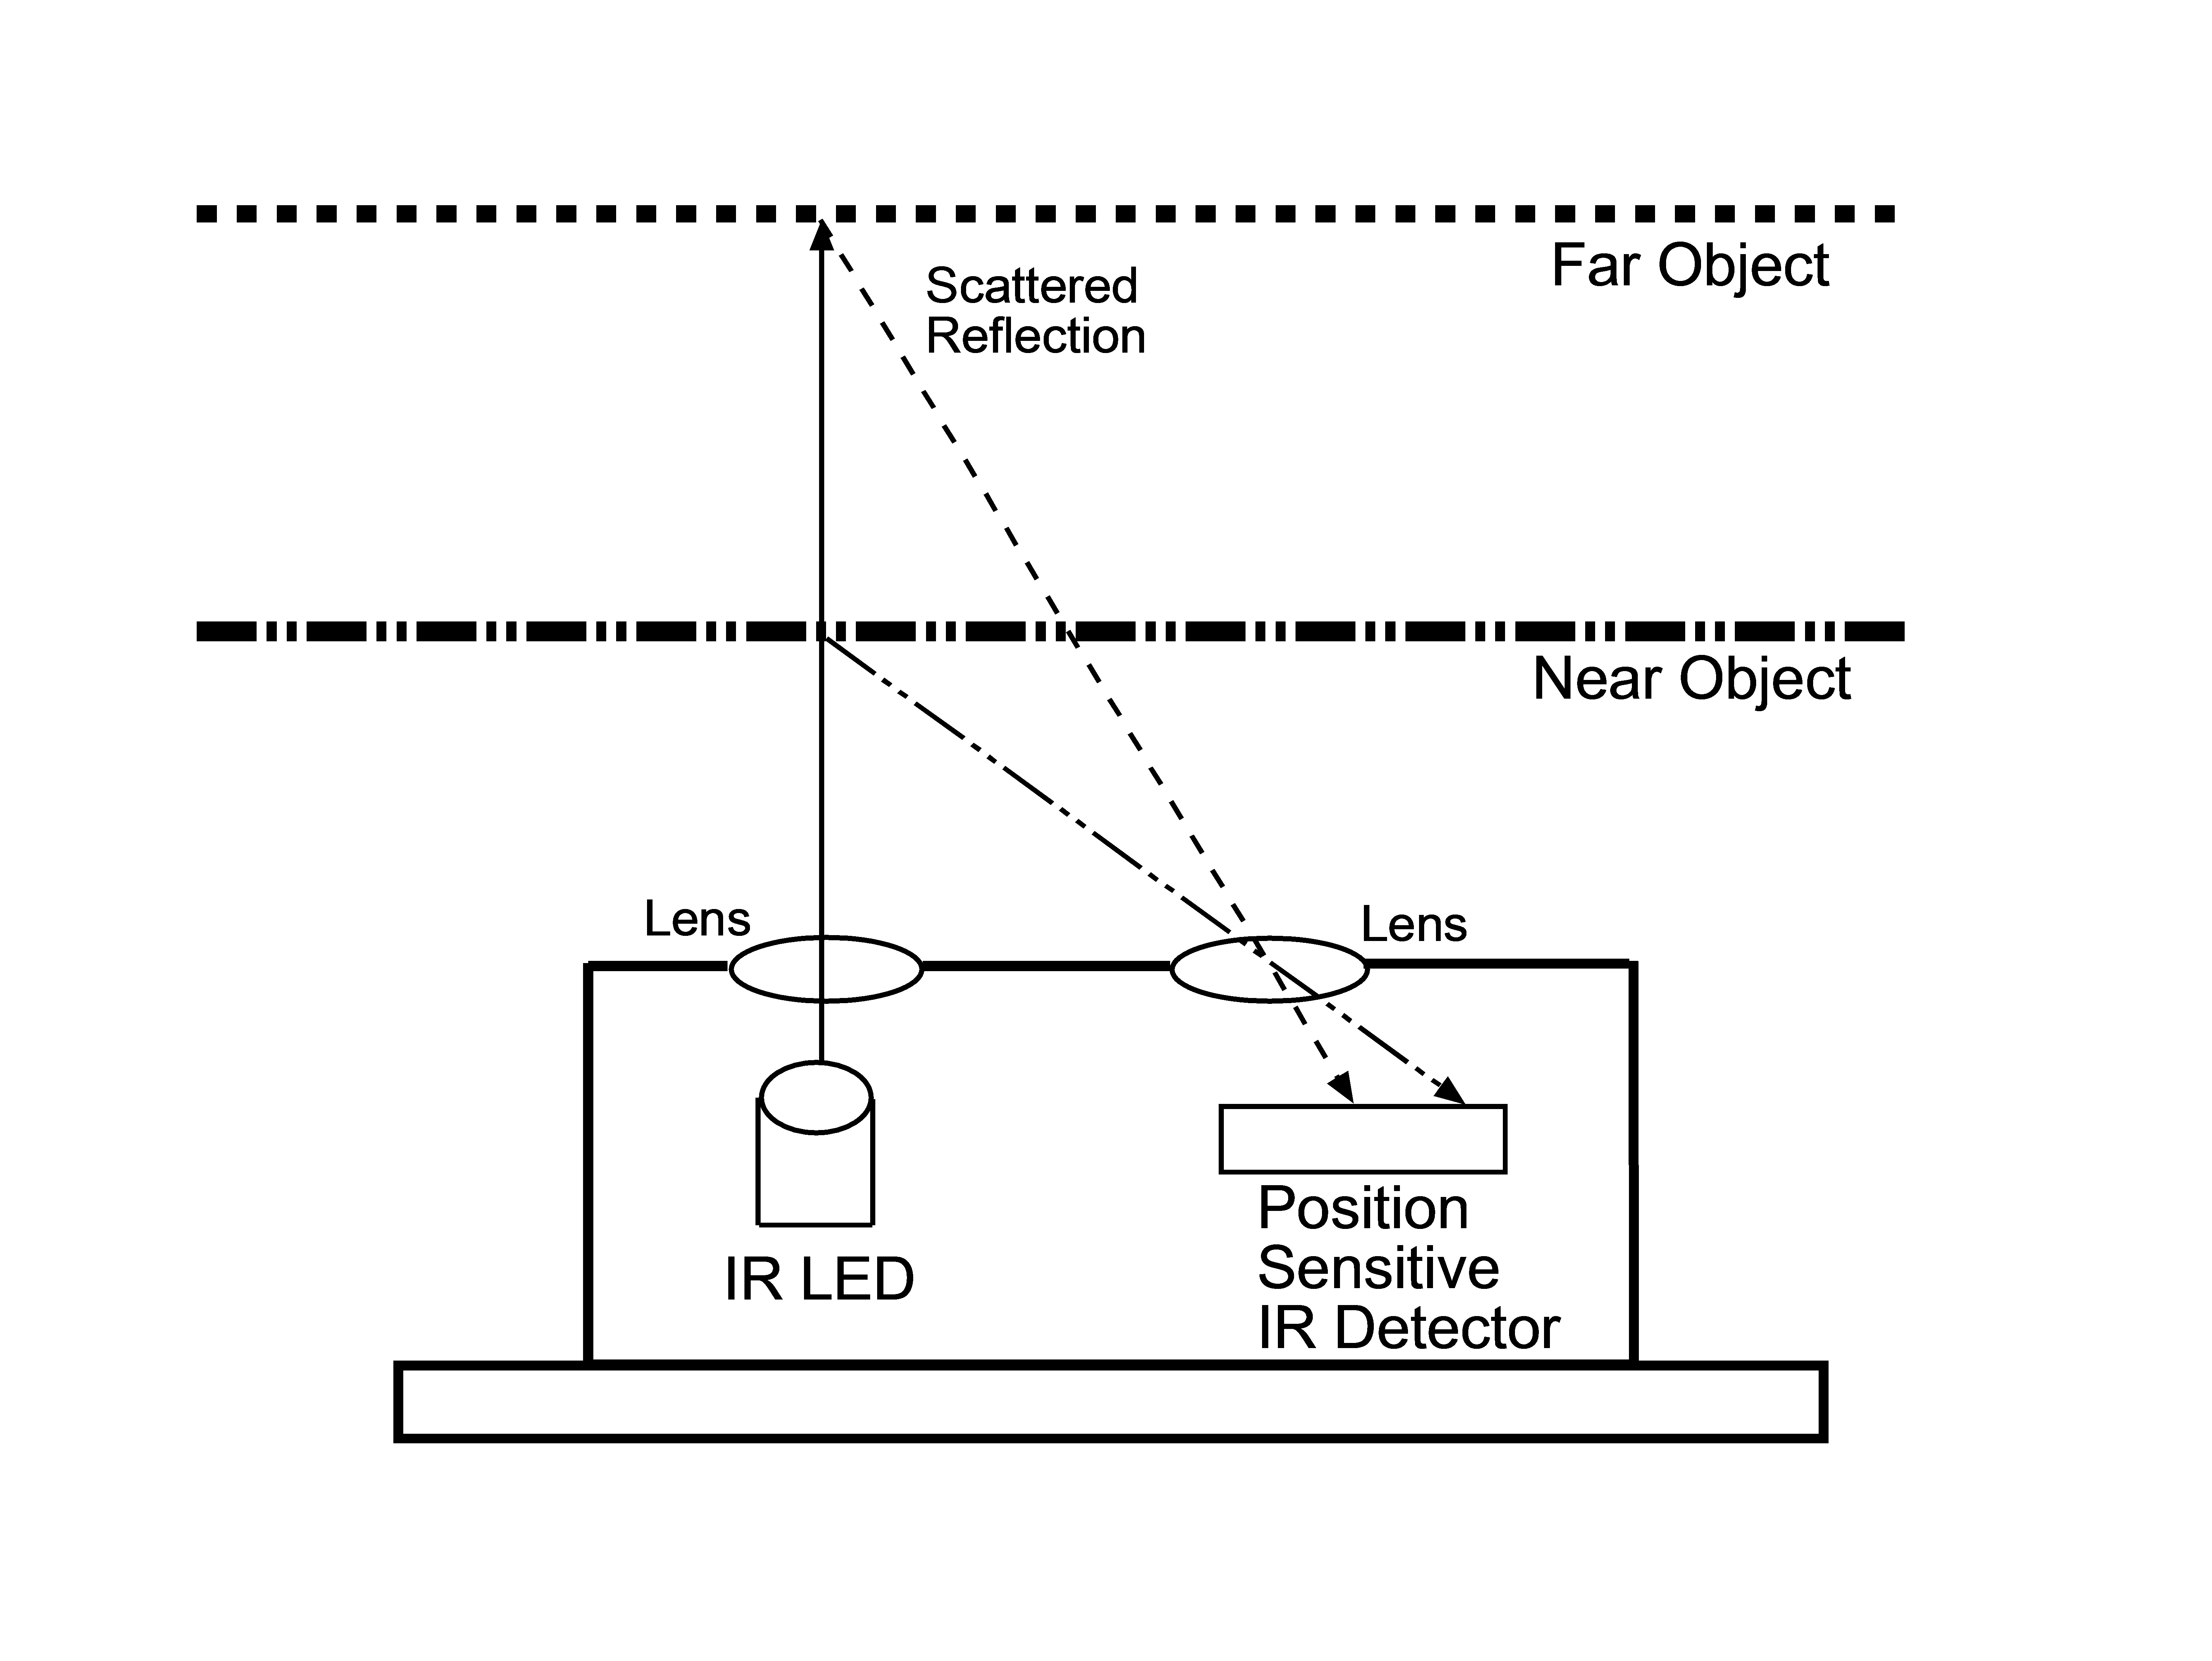
\includegraphics[width=.6\linewidth]{images/rangefinder.jpg}
	\caption{A slightly more complex laser rangefinder.}
	\label{fig:rangefinderIMG}
\end{figure}

In this picture we see a different setup for a rangefinder. Instead of measuring the time it takes for the pulse to get back, it measures the distance between where the pulse was emmited, and where it was absorbed. Given this distance, and the fact that the pulse is emmited at a right angle to this distance, simple trigonometry can be used to determine the distance the pulse travelled.

It is required that rangefinders know what the speed of the pulse is, which is a problem in unknown environments. For a rangefinder to be reliably used in such environments, it needs either to have the speed of its pulse pre-calculated, or it needs to measure the speed of the pulse by itself. Also, in situations where the speed of the pulse varies, a rangefinder is either not useful, or it needs a more complicated model of the environment it is in.

The main cause for a pulse to travel at a different speed than expected is in situations where the environment the sensor is in varies in density, which depends on temperature\cite{refraction}. Hence, a simple rangefinder is not fit for an environment that varies heavily in temperature.

Sound moves faster through denser mediums, where light travels slower. The speed of light is less affected by density than sound is. In earth-like atmospheres, light only travels 0.03\% slower in air when compared to the vacuum.\cite{refraction}\cite{speedOfSound}.

Another issue in environments with a high variation in density is refraction. Refraction is a phenomenon that occurs when a wave switches between mediums where it travels at different speeds. This change causes the wave to change its direction\cite{snell}. Refraction would cause rangefinders to become effectively blind, as neither their direction nor the length measured can be trusted.

\begin{figure}[H]
	\centering
	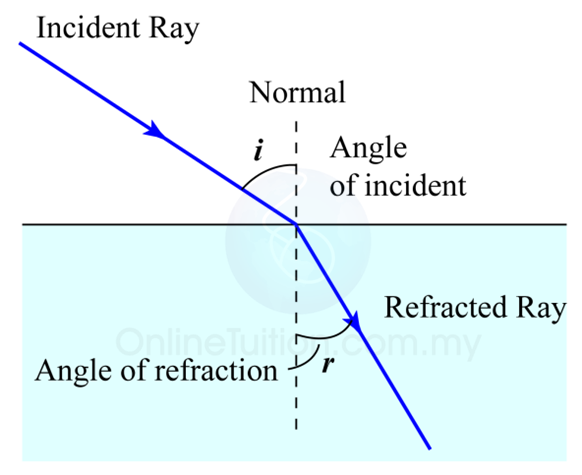
\includegraphics[width=.4\linewidth]{images/refraction.png}
	\caption{An illustration of refraction into a denser medium.}
	\label{fig:refractionIMG}
\end{figure}

We can categorize reflectivity of an object or surface into three categories:\cite{reflectivity}

\begin{itemize}
	\item Diffuse reflective
	\item Specular
	\item Retro-reflective
\end{itemize}

Just to expand upon these categories, it is possible to look at the reflective characteristics of an object's surface.

We find \textbf{diffuse reflective} objects to have a textured quality, which causes the reflected energy to disperse uniformly from the object. These materials tend to be read very well by a large number of laser sensors, due to the relatively predictable percentage of dispersed laser energy finding its way back to the laser receiver. Some examples of these objects would be: paper, granite and textured walls. It is important to note, that different wavelengths may exhibit unexpected results with certain receivers.

\textbf{Specular} objects or surfaces tend to not read very well, due to the emitted energy not being dispersed correctly. Examples of specular surfaces are glasses and mirrors.

With very reflective properties, we categorize objects and surfaces as \textbf{retro-reflective}. These usually return a very high percentage of emitted energy to the receiver, therefore are a good target to many lasers. Some examples would be: reflectors, license plates and animal eyes.

\subsection{Autonomous Vehicles and Robots}

Autonomous robots or vehicles can work for an extended period of time, gathering information from its surroundings, while being able to work without human interaction. The robot or vehicle gathers different kinds of data, depending on what the goal of the device is. Positional data can be utilized for navigation and path finding in a known and unknown environment. Intelligent autonomous robots and vehicles are able to adapt to changes happening in its surroundings. Currently there are many robots on the market that are self-reliant, ranging from autonomous vacuum cleaners to drones and helicopters\cite{autonomousbasic}.

Simple autonomous robots use ultrasonic sensors or infrared LEDs to manipulate its own behaviour, if it detects obstacles or unexpected scenarios in the environment. This is useful for obstacle-avoidance and mapping of unknown areas, where the robot, through different reference points, can pin-point the obstacles it has encountered along the way and in the future, more efficiently avoid them.
More advanced robots use more advanced vision to grant them the ability to see their surroundings. Algorithms then analyse the vision data and gives the robot a depth perception, which grants the ability to instantly identify objects and locate them and memorize them accordingly\cite{obstacles}.

There are two main kinds of autonomous robots: a single computer-autonomous robot and insect robots. The single-computer autonomous robot uses its own on-board computing unit to do its computations and its decisions, whereas the insect robots are a fleet of many smaller robots, which are controlled by a single and separate computing unit. The advantage of having a single-computer autonomous robot is that the tasks it performs can be done using more dedicated computer resources. It has the possibility of utilizing the computing power to its full potential, instead of relying on a separate unit that is also making decisions and calculations for many other robots. The insect robots are usually fairly simple in terms of capabilities, but the whole robot fleet can be utilized to perform advanced and possibly more sophisticated tasks, that requires a fleet simpler robots designed to work together autonomously\cite{singleandinsect}.

\subsection{Pathfinding and Mapping}

Pathfinding is done by a computer, where it uses plotting to find the shortest path between two different points. It can be viewed as an efficient way of navigating a maze. The main objective is getting from some location to a goal location.
There are different pathfinding algorithms already existing that are used for software simulations, but also for mobile robot navigation. Common pathfinding algorithms are A* (pronounced A star) and its extended version named D* (Dynamic A*).

\begin{figure}[H]
	\centering
	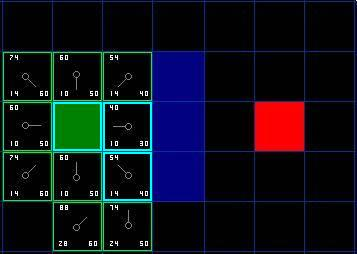
\includegraphics[width=.7\linewidth]{images/aStar2.jpg}
	\caption{Upper-left number is F, Lower-left G and Lower-right H}
	\label{fig:sub2}
\end{figure}

The A* algorithm is most commonly used in video games. The algorithm splits a known map into nodes (these can be any geometric shape, for example squares), and assigns a cost between each node. It also notes which nodes cannot be moved to, such as pits or walls. Based on this map, it determines the cost of movement from its position to some adjacent node(G), and estimates the cost of movement from that node to its final destination(H). It assigns this node with the value F which is the sum of G and H. It continues checking adjacent nodes with the same procedure, occasionally changing the calculated path based on the F values of various nodes\cite{astar}.

In the early stages of robot automation, it was always assumed that the environment around the robot was known and the path was generated based on this. This was okay until the robot was introduced to the unknown, and then started to meet inconsistencies and obstacles in its path (this being discrepancies between the true state and the world state), the robot then either had to re-plan completely from scratch or alter the plan through trial-and-error. Computational wise, it would require too much power to re-plan from scratch (Even though this is the optimal choice) and most of the time trial-and-error does not yield an optimal outcome.

\begin{figure}[H]
	\centering
	\begin{subfigure}[H]{0.4\textwidth}
		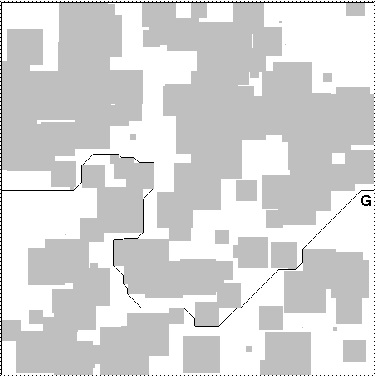
\includegraphics[width=\textwidth]{images/completemap.jpg}
		\caption{Complete Map}
		\label{fig:completemap}
	\end{subfigure}%
	\quad
	\begin{subfigure}[H]{0.4\textwidth}
		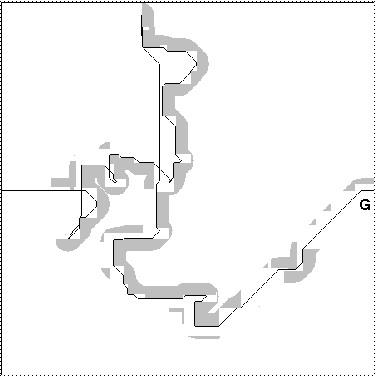
\includegraphics[width=\textwidth]{images/optimisticmap.jpg}
		\caption{Optimistic Map}
		\label{fig:optimisticmap}
	\end{subfigure}
	\caption{Mapping simulations with D*\cite{dstar}}
\end{figure}

The D* algorithm creates an initial path, based on assumed and known information. It then edits the path based on new information it receives whilst navigating the path. The final version of the edited plan is equivalent to re-planning the whole thing from scratch, but avoiding the limitations of the computation power.
Whenever an on-board sensor receives information about an obstacle, the algorithm can edit the path based on what possible routes there are available near-by.
D* is fast at navigating large scale unknown environments because during its exploration it is able to edit and repair its desired path and navigate towards its goal. It would require too much effort to re-plan everything from scratch every time it failed, especially for large scale environments\cite{dstar}\cite{moredstar}.

Figure \ref{fig:completemap} shows the map where the given robot knows its environment (the gray boxes) and can therefore easily determine the optimal path or the \textit{Complete Map} in this case. Figure \ref{fig:optimisticmap} on the other hand shows the \textit{Optimistic Map}, since before navigating on the planned path it assumes that there are no obstacles. Whenever the robot meets an obstacle during the optimistic map, it adjust its course to continue towards its goal. On figure \ref{fig:optimisticmap} it only displays the obstacles which the robot met during its journey  along the path.

Simple autonomous robots navigate by the use of infrared LEDs or photo-resistors and LEDs, by following lines drawn on a surface. Robots that use photo-resistors to follow a line are continuously looking for a change in brightness of the surface. If a line-following robot is tracking a black line, then whenever the photo-resistor picks up the brightness from the surface that is not a black line, the path will change accordingly. A large number of photo-resistors can be used to increase the intelligence of an autonomous line-following robot, since the greater amount of LEDs can detect intersections between lines and different routes and be identified\cite{linetrack}.\\
Some autonomous robots and vehicles use multiples of different range-sensors and other sensory equipment, to map and locate themselves in indoor and outdoor environments. The map that is generated can be used to keep track of static items in the environment such as structures and difference in terrain, but the map can also distinguish non-static items such as humans and other moving objects, from the static items. Since the maps are created by the vehicle itself whilst exploring, this technology can be used in places where there are no reference points, such as GPS\cite{rangesens}\cite{rangesensarc}. Robots and vehicles have been created using this technology to explore known and unknown environments. Because of advanced algorithms and hardware these autonomous devices are capable of performing some tasks more efficiently than humans, but are also able to perform them in places that are unsafe and hard to reach.

Autonomous robots also use these tools to work together. Using a shared map, the robots can keep track of one another and either perform tasks together or separately, depending on what is required from them.

\begin{figure}[H]
	\centering
	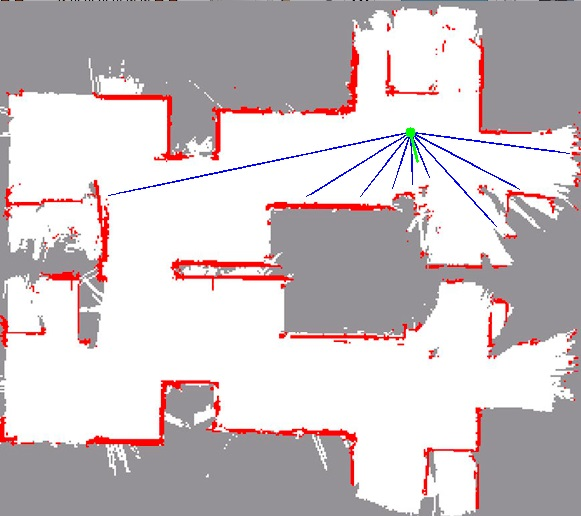
\includegraphics[scale=.7]{images/laserrangemap.jpg}
	\caption{Laser Range Map\cite{laserrangepic}}
	\label{fig:laserrangemap}
\end{figure}

Laser-range finders and sonar arrays are used to navigate and determine the shortest possible path to a given destination. The sensory equipment is used to give the autonomous robot a sense of distance towards objects in an environment, giving it vital data regarding optimal travel directions and information on how to avoid obstacles\cite{lasersonar}.

\subsection{Resources}
For the purpose of exploration and resource gathering, planets can be split into two categories. These two categories are:\cite{planettypes}
\begin{itemize}
	\item{\textbf{Terrestrial planets}, also known as the \textit{Inner Planets}}
	\item{\textbf{Gas giants}, also known as the \textit{Jovian planets} or the \textit{Outer Planets}}
\end{itemize}

There is very little reason to explore a gas giant, as they smoothly transition between gas, liquid, and solid. This means that it is extremely difficult to colonize such a planet, or build anything on it for that matter, due to the layers of condensed helium and hydrogen that make out their atmosphere\cite{outerplanetatmosphere}.
On the other hand, Earth-like planets have a larger variety of resources, and it is easier to build upon them. These planets are often composed largely of metals and silicon, which is what gives them their rocky and sandy surfaces.

\subsection{Environment}
\subsubsection{Atmosphere}
There are quite a few planets, in our solar system, with a negligible atmosphere. On these planets sound based sensors cannot work, but light based ones might even work better. These planets also tend to have a temperature very close to absolute zero\cite{planetstemp}.
Planets with an atmosphere can be much harder to cope with. On these planets there can be threats such as, high-winds, high-pressure, high-temperatures, corrosive gases, and liquids. When designing equipment for such environments, the specific environment must be kept in mind.

\subsubsection{Terrain}
Earth-like planets are, by definition, rocky/sandy planets, which tend to have mountains, canyons, and craters.
Earth-like planets do not have a very big variation in terrain, as most of them do not have any liquid substances that could change the terrain.
